%%% PREAMBLE - Do not touch %%%%%%%%%%%%%%%%%%%%%%%%%%%%%%%%%%%%%%%%%%%%%%%%%%%%%%
\documentclass[10pt,twocolumn,letterpaper]{article}
\usepackage[utf8]{inputenc}
\usepackage[english]{babel}
\usepackage{bm}
\usepackage{model}
\usepackage{times}
\usepackage{epsfig}
\usepackage{graphicx}
\usepackage{amsmath}
\usepackage{amssymb}
\usepackage{color}
\usepackage[pagebackref=true,breaklinks=true,letterpaper=true,colorlinks,bookmarks=false]{hyperref}
\input{pics/abaco}

\cvprfinalcopy % *** Uncomment this line for the final submission
\def\httilde{\mbox{\tt\raisebox{-.5ex}{\symbol{126}}}}
\ifcvprfinal\pagestyle{empty}\fi


%%% Report beginning %%%%%%%%%%%%%%%%%%%%%%%%%%%%%%%%%%%%%%%%%%%%%%%%%%%%%%%%%%%%%%
\begin{document}

%%% Title and authors %%%%%%%%%%%%%%%%%%%%%%%%%%%%%%%%%%%%%%%%%%%%%%%%%%%%%%%%%%%%
\title {Predicting the number of shares of a social network with linear regression }
\author{Gustavo Ciotto Pinton, RA117136\thanks{Is with the Institute of Computing, University of Campinas (Unicamp). \textbf{Contact}: \tt\small{gustavociotto@gmail.com}}}

%%% Abstract %%%%%%%%%%%%%%%%%%%%%%%%%%%%%%%%%%%%%%%%%%%%%%%%%%%%%%%%%%%%%%%%%%%%%
\maketitle
\begin{abstract}
Relying on a Mashable social network's real database \cite{database}, this report uses linear regression techniques to predict the number of shares that an eventual publication would have based on its describing features. Improving tools such as regularization and variable selection are explored, and the settings of their important parameters are discussed as well. The proposed linear regression was obtained by two different methods, gradient descent and least squares, whose results are compared in the last sections of this document.
\end{abstract}

%%% Introduction %%%%%%%%%%%%%%%%%%%%%%%%%%%%%%%%%%%%%%%%%%%%%%%%%%%%%%%%%%%%%%%%%
\section{Introduction}
\label{intro}

Linear regression consists of a simple technique whose objective is to relate an input data set to a output data set through the use of a linear equation \(Y = \theta_0 + \theta_1X_1 + \theta_2X_2 + \ldots + \theta_NX_N\), in which \(Y\), \(X_i\) and \(\theta_i\) represent, respectively, the output generated by the model from a set of describing attributes and the coefficients of the equation. The previous equation is used only for a singular sample, but, as seen in class, one of the main aspect that guarantees the quality of results obtained by machine learning methods is the large volume of data. Having that in mind, a set of \(M\)  input samples described by \(N\) attributes is represented by the matrix \(\bm{x}_{N+1\times M}\).  In the same way, the coefficients of the equation are represented by the vector \(\bm{\theta}\) of \(N+1\) elements and the output by the vector \(\bm{y}\) of size \(M\), in order to obtain the vector equation \ref{lr}, just below.

\begin{equation}
\label {lr}
\bm{y} = \bm{\theta}^T\bm{x}
\end{equation}

The determination of each component of \(\bm{\theta}\) is performed through the minimization of the cost function \(J(\bm{\theta}, \bm{x})\), described by the equation \ref{cost}, in which \(\bm{x}_ i\) corresponds to the i-th sample and \(t_ i\) to the \textit{target} that we want to achieve.

\begin{equation}
\label {cost}
J(\bm{\theta}, \bm{x}) = \frac{1}{2M} \displaystyle\sum_{i=1}^{M} \left(\bm{\theta}^T\bm{x}^{(i)} - \bm{t}^{(i)}\right)^2
\end{equation}

The datasets used during the minimization process,  \(\bm{x}\) and \(\bm{t}^{(i)}\), belong to a set called \textbf{training set}, meanwhile the parameters and model validation occurs in a set that receives this same name. A general rule is to use at least 80\% of the available data for training and the rest, 20\%, for testing and validation.

The cost function \(J(\bm{\theta}, \bm{x})\) has the important property of being  \textbf{convex} \cite{Bishop:2006:PRM:1162264}. This fact ensures that it has no local minima, except for the global one. Thus, two minimization methods can be used. The first one, called \textbf{normal equations},  allows to obtain the optimal \(\bm{\theta}\)  from a single expression, represented in \ref{normal}. It is quickly verified that the negative point of this approach is the calculation of the inverse matrix, whose asymptotic computing complexity is \(\Theta(n^3)\), as seen in class. For the matrix \(\bm{x}^T\bm{x}\) of dimension \(N+1 \times N+1 \), the number of attributes \(N\) may represent an impediment to the use of this technique.

\begin{equation}
\label {normal}
\bm{\theta} = \left(\bm{x}^T\bm{x}\right)^{-1} \bm{x}^T \bm{t}
\end{equation}

The second method, called \textbf {gradient descent}, is iterative and does not require the computing of any inverse matrix. By partially deriving the equation \ref{cost} in relation to \(\bm{\theta}_j\), it is possible to obtain the cost function slope and therefore the direction we must take to approximate the model to the global minimum. By repeating this reasoning for all parameters \(\bm{\theta}_j\), we obtain the operation \ref{gd} which must be applied to each of them at each iteration. It is emphasized that \(\bm{x}_1 = 1\) for all \(i\).

\begin{equation}
\label {gd}
\bm{\theta}_j = \bm{\theta}_j - \alpha\frac{\partial J}{\partial \bm{\theta}_j } = \bm{\theta}_j - \frac{\alpha}{M} \displaystyle\sum_{i=1}^{M} \left(\bm{\theta}^T\bm{x}^{(i)} - \bm{t}^{(i)}\right)\bm{x}_j^{(i)}
\end{equation}

Equation \ref {gd} introduces the parameter \(\alpha\), called \textit {learning rate}. This parameter controls the convergence speed to the global minimum, i.e, the higher its value, the faster it is reached. On the other hand, very large values will produce an effect called \textit {overshooting}, that is, the found solution will always \textit {swing} around the minimum without ever reaching it. In the following sections, the author explains the strategy he used to define this parameter for this problem.

Having seen all the theory behind linear regression, we can now apply it to the real datasets. In this report, it is used a real database \cite {database} got from the \textit{Mashable} social network, which relates a series of attributes of a given publication to the number of shares it has received. In other words, it is sought to find a linear relationship between the number of shares received with the attributes of a publication. In total, 31715 input samples were used to train and validate the models and 7929 for testing.

%%% Add section %%%%%%%%%%%%%%%%%%%%%%%%%%%%%%%%%%%%%%%%%%%%%%%%%%%%%%%%%%%%%%%%%%
\section{Activities}

The next subsections explain the choices of the various parameters adopted by the author.

\subsection{Learning rate setting strategy}
\label{sec:ajuste}

As mentioned in the \ref{intro} section, the learning rate parameter controls the speed of convergence to the cost function's global minimum. Considering the issues discussed in this same section, an initial \(\alpha\) value of 0.5 is adopted, modifying it in only two situations:

\begin{itemize}
	\item When the error at iteration \(k\) is greater than the one of the iteration \(k -1\). In this case, it is concluded that the solution found was worse and, therefore, we must decrease the speed of convergence to avoid the solution to keep \textit{swinging} around the minimum.
	\item The error variation between iterations \(k\) and \(k -1\), i.e., \(\frac{R_{k-1} - R_k}{R_k}\), was less than a percentage \(\Delta = 0.5\%\). In this case, it is desired to eliminate the effects of \textit {overshooting} and to bring the solution as close as possible to the global minimum. The root mean square error obtained at iteration \(k\) is denoted by \(R_k\) and given by the formula \ref {rms}:
	\begin {equation}
	\label{rms}
	R_k = \sqrt{\frac {\sum_{i=1}^{M} \left(\bm{\theta}_k^T\bm{x}^{(i)} - \bm{t}^{(i)}\right)^2}{M}}
	\end{equation}
\end{itemize}

In these two situations, the value of \(\alpha\) is divided by half.

\subsection {Adjustment of the discrete variables}

The attributes description of each of the entries revealed the presence of some discrete variables. Two groups were identified: one with variables of type \textit {publication occurred on Monday?}, \textit {publication occurred on Tuesday?} and so on, and one with attributes similar to \textit{is an entertainment channel?}. Before using them or not in the models proposed below, it is necessary to verify if such variables are \textbf {orthogonal} to each other, that is, if the distance between them considered two by two is always the same. Taking into account that the variables of both groups can never be set simultaneously (a publication can not occur on Monday and Tuesday and it can not belong to two channels at the same time, for example), we can verify the property of \textbf {orthogonality} and therefore we can use them without any modifications.

\subsection {Input and output data sets normalization}

The normalization of the dataset before training prevents the values \(\bm{\theta}_j \) being extremely small or large, causing instabilities or interferences in the model's convergence speed. Among the many ways of normalization that can be applied, we choose for this activity the one of equation \ref {norm}. In this case, the mean \(\mu_j\) and the standard deviation \(\sigma_j\) of each feature are calculated over all training samples and then the expression \ref {norm} is applied.

\begin {equation}
\label {norm}
\bm {x'}_j = \frac {\bm{x}_j - \mu_j}{\sigma_j}
\end{equation}

Note that the values \(\mu_j\) and \(\sigma_j\) must be saved for later use in the test set or any other input to be used with the model.

\subsection{Regularization}

\label{sec:reg}

Regularization is a technique that allows to limit the negative effects of \textit{overfitting} without removing any describing feature from the model. It consists of applying a penalty factor over each parameter \(\bm{\theta}_j \). Equation \ref{cost} then becomes:

\begin{equation}
\label {cost-reg}
J(\bm{\theta}, \bm{x}) = \frac{1}{2M} \left[\displaystyle\sum_{i=1}^{M} \left(\bm{\theta}^T\bm{x}^{(i)} - \bm{t}^{(i)}\right)^2 + \lambda \displaystyle\sum_{j=2}^{N + 1} \bm{\theta}_j^2 \right]
\end{equation}

If \(\lambda\) is very large, then the minimization process will produce a small-norm vector \(\bm{\theta}_j\), resulting in a biased model that would not succeed in fitting to the training data. In contrast, small \(\lambda\) could not counteract the effects of \textit {overfitting} and the variation created by the test dataset would still be large.

Equation \ref {norm}, in turn, becomes expression \ref{normal-reg}, where \(\bm{I}_{N \times N}\) is the identity matrix:

\begin{equation}
\label {normal-reg}
\bm{\theta} = \left(\bm{x}^T\bm{x} + \lambda
\begin{bmatrix}
    0       & 0 \\
    0       & \bm{I}_{N \times N} \\
\end{bmatrix}
\right)^{-1} \bm{x}^T \bm{t}
\end{equation}

Note that \(\bm {\theta}_1 \), the bias appended into the model, is not penalized.

%%% Add section %%%%%%%%%%%%%%%%%%%%%%%%%%%%%%%%%%%%%%%%%%%%%%%%%%%%%%%%%%%%%%%%%%
\section{Proposed solutions}

This section is dedicated to discussing the proposed solutions. We performed tests with simple, regularized and containing second and third order variables models. For the gradient descent technique, the input dataset was randomically divided into two other sets, training (70\%) and validation (30\%). For the normal equations, no further separation was applied to the original training dataset.

\subsection {Simple linear model}

In this model, the linear regression method is used without any regularization factor and second or third order terms. For the gradient descent technique, the formula \ref {gd} is computed in a loop that iterates 100 times in total. Figure \ref {fig:lr-gd} represents the root mean square errors according to the equation \ref{rms} obtained for the training, validation and  test datasets at each iteration. It is observed that both errors stabilize around 11357 and 14638 respectively and that there were no negative effects of overfitting. Curiously, the obtained validation error curve is below the curve corresponding to the training dataset during almost all the simulation.

\begin{figure}
    \centering
    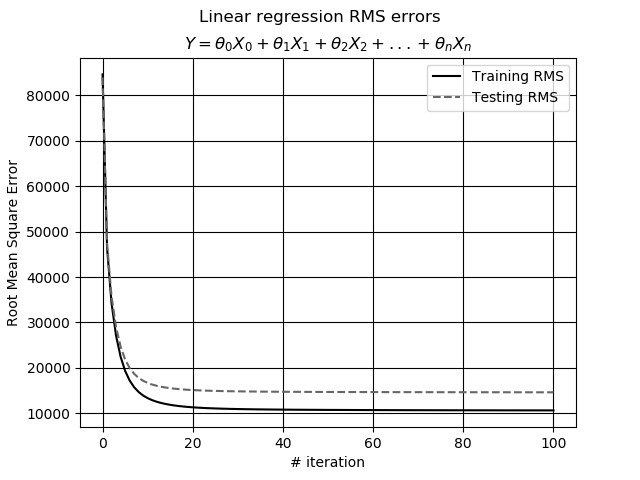
\includegraphics[width=0.9\columnwidth]{img/lr-gd.png}
    \caption{Training and test errors obtained at each iteration.}
    \label{fig:lr-gd}
\end{figure}

Figure \ref{fig:lr-norm}, in turn, represents the results found through the use of the expression \ref{norm}. Two plots are shown: in the first one, we compare the errors obtained in the train and test datasets for many input set sizes ranging from 10000 to 31715, meanwhile in the second, we compare the parameter vectors \(\bm{\theta}\) obtained by the two methods described in this section. As expected, the RMS found by the normal equation, around 10580, was lower than the one found by the \textit {gradient descent} technique. The test error, in turn, also remained around 14570. It is also noted that there are some considerable differences between the vectors \(\bm{\theta}\) computed by each method, especially for intermediate sized data sets. In order to have a better comparison for quality among the final results, we use the mean absolute error (MAE). This metric tells the absolute average difference between the shares that a publication received and the one predicted. For the normal equations, the mean absolute errors for training and test are 3005 and 3183, respectively. This means that for a given publication, our model is predicting in average either 3000 more or less shares.

\begin{figure}
    \centering
    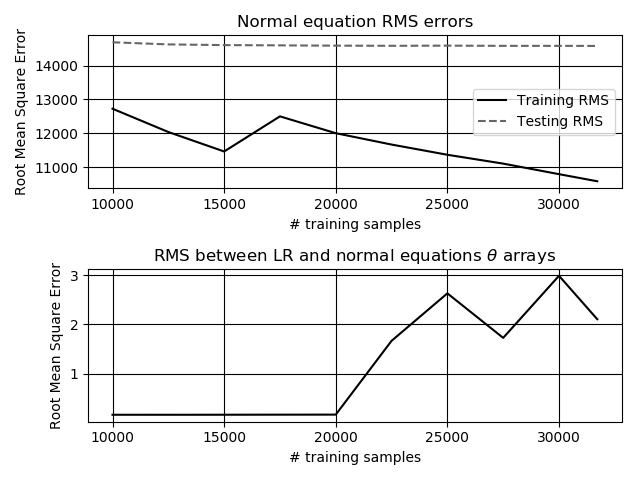
\includegraphics[width=0.9\columnwidth]{img/lr-norm.png}
    \caption{Training errors obtained for many dataset sizes.}}
    \label{fig:lr-norm}
\end{figure}

\subsection{Regularized simple linear model}

Although we have not verified the \textit{overfitting} presence in the previous results, we propose the use of regularization, as explained in subsection \ref{sec:reg}. Two values of \(\lambda\) were tested, one equal to 1.0 and the other, twenty times greater, 20.0. Figure \ref{fig:reg-comparison} compares the results found by the \textit{gradient descent} technique between the regularized model and the one from the previous subsection. We verify that the regularization did not substantively modify the error found for both the training and the test sets. This indicates that the suggested values of \(\lambda\) are not big enough when compared to each of the factors \(\bm{\theta}_j^2 \) individually to produce changes on the model. These same models were also submitted to the normal equations, however, as in the \textit{gradient descent}, no considerable changes were noted.

\begin{figure}
    \centering
    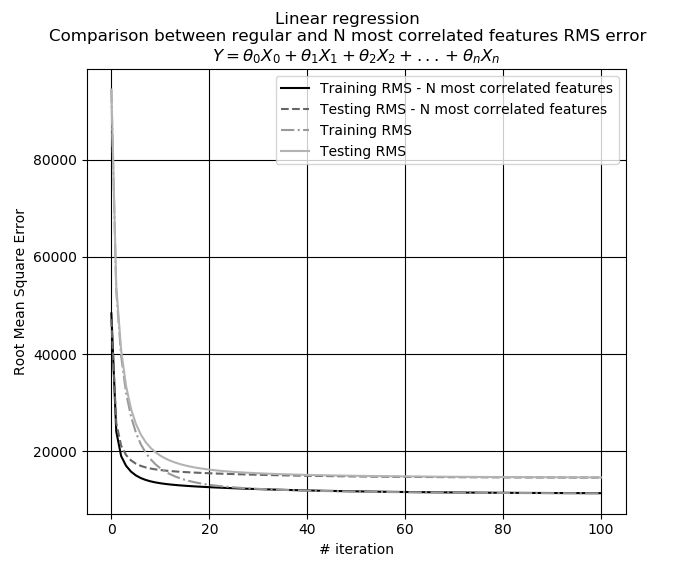
\includegraphics[width=0.9\columnwidth]{img/lr-comparation.png}
    \caption{Training and test errors obtained by the regularized models.}
    \label{fig:reg-comparison}
\end{figure}

\subsection{Reduction of features}

Another attempt to minimize the error consisted of reducing the number of attributes used in the model. The attributes selection was done by computing the correlation of each of them to the output. Considering that the model is still linear, it is expected that more correlated variables follow the same pattern as the one observed at the output. The figure \ref{fig:correlation} represents only the 10 most correlated variables that were used for the proposed new model. It is worth mentioning that the highest correlation, corresponding to attribute 27 (\textit{Avg. Keyword (avg. Shares)}), is still a very low value, i.e, 0.125, indicating that no variable strongly influences the number of shares received by a publication. Figure \ref {fig:comparison-selection} compares the results found by the simple linear model and the model proposed in this subsection. A very slight increase in the testing error for the reduced model is observed at the iteration 10, indicating a slight overfitting presence. In addition, it is verified that both training and test errors of the reduced model converge faster than those computed by the simple model. Finally, the mean absolute errors verified by the normal equation for the training and test datasets were 3016 and 3195, respectively.

\begin{figure}
    \centering
    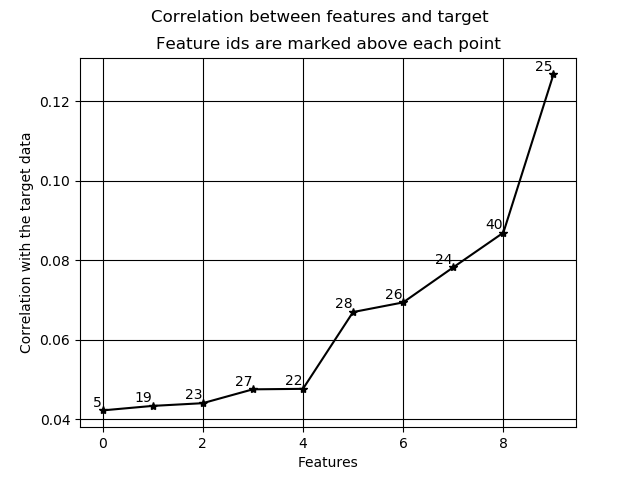
\includegraphics[width=0.9\columnwidth]{img/lr-selection.png}
    \caption{Correlation of the input features with the output.}
    \label{fig:correlation}
\end{figure}

\begin{figure}
    \centering
    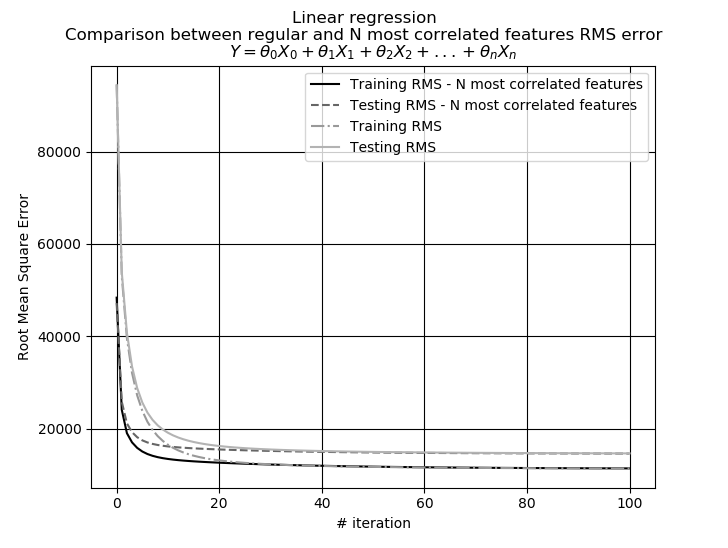
\includegraphics[width=0.9\columnwidth]{img/lr-comparation-selection.png}
    \caption{Comparison between simple linear model and the one with the 10 most correlated variables with the output.}
    \label{fig:comparison-selection}
\end{figure}

\subsection{Linear model with second order attributes}

Another technique that can be used to reduce training and test errors is the addition of new attributes based on the existing ones to the simple model. In this case, we append to the traning and test input datasets all existing variables to the power of 2, obtaining the new relation \(Y_2 = Y + \theta_{N + 1}X_1 ^ 2 + \theta_{N + 2}X_2 ^ 2 + \ldots + \theta_{2N}X_N^2\). This new model is expected to be better adapted to the training and test data simultaneously, i.e, without overfitting. Note that the equations \ref{normal} and \ref{gd} do not need to be changed, given that the cost equation \ref {cost} remains linear in \(\bm{\theta}\). Figure \ref{fig:gd-second} has the result of the \textit {gradient descent} technique for this new model. Note that at iteration 5, the value of \(\alpha\) is modified, as described in section \ref{sec:ajuste}, since the error produced was higher than that found in the previous iteration. The training and test RMS errors after 100 iterations were, respectively, 13317 and 17089, higher than those verified for the simple linear model. The use of the \ref{normal} equation, in turn, resulted in errors around 10540 and 14580, very similar to those obtained by the same technique applied to the simple linear model. Finally, the mean absolute errors verified by the normal equation for the training and test datasets were 3001 and 3183, respectively.

\begin{figure}
    \centering
    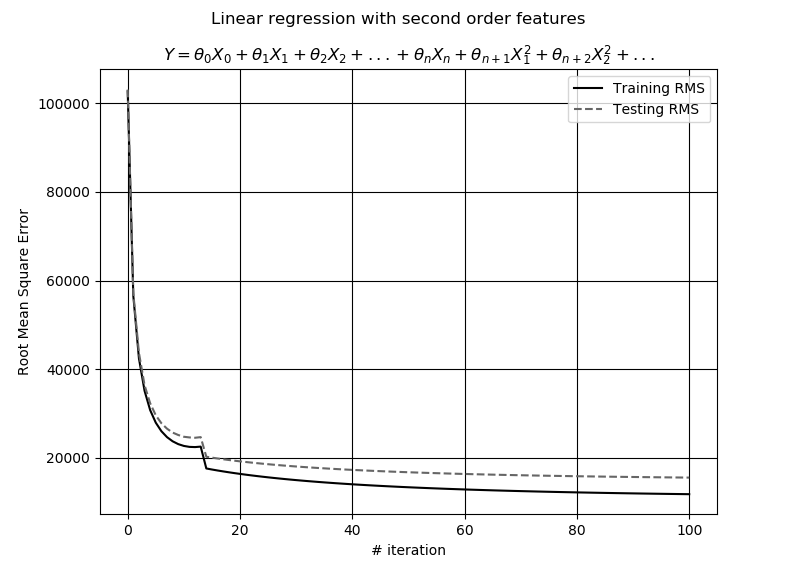
\includegraphics[width=0.9\columnwidth]{img/lr-second-gd.png}
    \caption{Training and test errors obtained at each iteration by the model with second order attributes.}
    \label{fig:gd-second}
\end{figure}

\subsection{Linear model with third order attributes}

The last model tested in this report used second and third order attributes, obtaining the expression \(Y_3 = Y_2 + \theta_{2N + 1}X_1 ^ 3 + \theta_{2N + 2}X_2 ^ 3 + \ldots + \theta_{3N}X_N^3\). The figure \ref{fig:gd-third} has the evolution of the errors found during the 100 iterations. As occurred in figure \ref{fig:gd-second}, the value of the parameter \(\alpha\) - the learning rate - had to be decreased considering that the training error of iteration 3 was higher than the one of the iteration 2. The smallest RMS errors found for training and testing were, respectively, 12990 and 16934, higher than those obtained in the simple linear model. Finally, the use of the normal equations resulted in errors equal to 10458 and 15084. The first was slightly lower than the same of the simple model, while the second, bigger. This fact illustrates one of the main difficulties encountered when we increase the complexity of the model: \textit{overfitting}. In this case, the error of the training set is reduced, but that one of test set is increased, indicating that the model has adapted in an exaggerated way to the training data. As already discussed, one of the possible solutions to this problem is regularization.

\begin{figure}
    \centering
    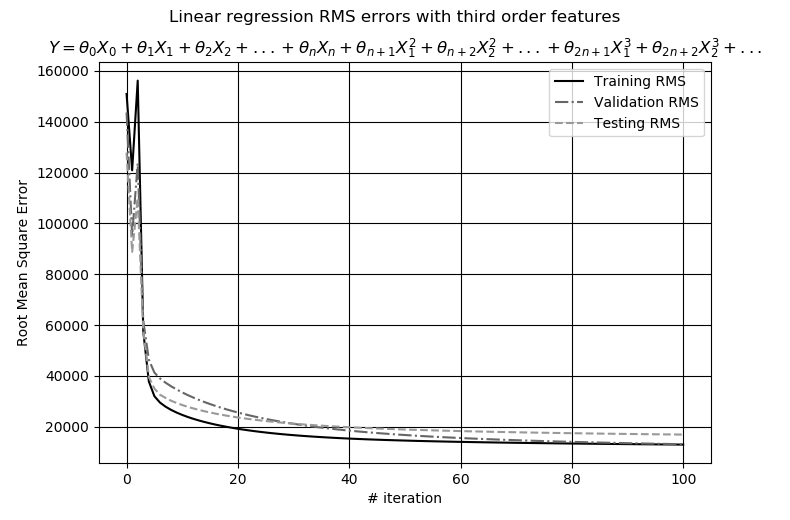
\includegraphics[width=0.9\columnwidth]{img/lr-third-gd.png}
    \caption{Training and test errors obtained at each iteration by the model with second and third order attributes.}
    \label{fig:gd-third}
\end{figure}

%%% Add section %%%%%%%%%%%%%%%%%%%%%%%%%%%%%%%%%%%%%%%%%%%%%%%%%%%%%%%%%%%%%%%%%%
\section{Conclusions}

Five linear models were proposed to predict the number of shares of a given Mashable social network publication. In almost all of them, the train and test mean absolute errors were around 3000 and 3180, respectively, indicating that the linear solution is not able to accurately model the behavior of the users of this social network. In other words, these errors mean that for any given publication, the proposed models are predicting almost 3000 more or less shares in average.

%%% References %%%%%%%%%%%%%%%%%%%%%%%%%%%%%%%%%%%%%%%%%%%%%%%%%%%%%%%%%%%%%%%%%%%
{\small
\bibliographystyle{unsrt}
\bibliography{refs}
}

\end{document}
